\documentclass[
%%%%% Styles and Sizes
%10pt,
%11pt,
%12pt,
fancyheadings, % headings with seplines and logo
%
%%%%% Printing, Color and Binding
%a4paper, 
%a5paper,
%twoside, % single sided printout
%oneside, % duplex printout (default)
%% binding correction is used to compensate for the paper lost during binding
%% of the document
%BCOR=0.7cm, % binding correction
%nobcorignoretitle, % do not ignore BCOR for title page
%% the following two options only concern the graphics included by the document
%% class
%grayscaletitle, % keep the title in grayscale
%grayscalebody, % keep the rest of the document in grayscale
%
%%%%% expert options: your mileage may vary
%baseclass=..., % special option to use a different document baseclass
]{stsreprt}

% Information for the Titlepage
\author{Robin Willenbrock}
\title{Static Detection of Data Races in Interrupt-Driven Software Using Reduced Inter-Procedural Control Flow Graphs}
\date{\today}
\subject{Bachelor Thesis}
\professor{Prof. Dr. Sibylle Schupp }
\advisor{Ulrike Engeln}

\usepackage[utf8]{inputenc}
\usepackage{listings}
\usepackage{amsmath}
\usepackage{xcolor}
% Font and Fontencoding Magic
% FAQ: 
% http://tex.stackexchange.com/questions/664/why-should-i-use-usepackaget1fontenc
% http://en.wikipedia.org/wiki/Computer_Modern
% http://tex.stackexchange.com/questions/1390/latin-modern-vs-cm-super
\usepackage[T1]{fontenc}
\usepackage{lmodern}
%\usepackage{fix-cm}
\lstset{
	language=Python,
	basicstyle=\ttfamily\footnotesize,
	keywordstyle=\color{blue},
	commentstyle=\color{green},
	stringstyle=\color{red},
	numbers=left,
	numberstyle=\tiny\color{gray},
	stepnumber=1,
	numbersep=5pt,
	frame=single,
	breaklines=true,
	showstringspaces=false,
	tabsize=4,
	captionpos=b
}
\usepackage{tikz}
\usetikzlibrary{shapes.geometric, arrows, positioning}
\usepackage{caption}
\usepackage{float}
\usepackage{adjustbox}
\usepackage[linesnumbered,ruled,vlined]{algorithm2e}
\raggedbottom

\tikzstyle{startstop} = [rectangle, rounded corners, minimum width=3cm, minimum height=1cm,text centered, draw=black, fill=red!30]
\tikzstyle{process} = [rectangle, minimum width=3cm, minimum height=1cm, text centered, draw=black, fill=orange!30]
\tikzstyle{decision} = [diamond, minimum width=3cm, minimum height=1cm, text centered, draw=black, fill=green!30]
\tikzstyle{arrow} = [thick,->,>=stealth]
\tikzstyle{redarrow} = [thick,->,>=stealth,draw=red]

% Package for Abbreviations
\usepackage{acronym}
\usepackage{hyperref} 

\begin{document}
	\frontmatter
	\maketitle
	\chapter*{Declaration of Originality\footnote{University of Tübingen, Department of Sociology}}
		Hereby I confirm, Robin Willenbrock, Matr. Nr. 53962,
		that this assignment is my own work and that I have only sought and used mentioned tools.
		\\
		I have clearly referenced in the text and the bibliography all sources used in the work (printed
		sources, internet or any other source), including verbatim citations or paraphrases.
		\\
		I am aware of the fact that plagiarism is an attempt to deceit which, in case of recurrence, can result in a loss of
		test authorization. 
		\\
		Furthermore, I confirm that neither this work nor parts of it have been
		previously, or concurrently, used as an exam work – neither for other courses nor within other
		exam processes.\\
		\\
		\\
		\noindent
		\begin{tabular}{@{}l@{}r@{}}
			Hamburg, July 10, 2024 & \hspace{5cm}\makebox[5cm]{\hrulefill} \\ 
			& \hspace{5cm}{\textit{Robin Willenbrock}} 
		\end{tabular}
	\tableofcontents
	\listoffigures{}
	\listofalgorithms
	
	% Abbreviations
	\chapter*{Abbreviations}
	\begin{acronym}
		\acro{ISR}{interrupt service routine}
		\acro{CFG}{control flow graph}
		\acro{ICFG}{inter-procedural control flow graph}
		\acro{RICFG}{reduced inter-procedural control flow graph}
		\acro{GCC}{GNU Compiler Collection}
		\acro{DFS}{depth-first search}
		\acro{BB}{basic block}
	\end{acronym}
	
	\mainmatter{
		\chapter{Introduction}
		Interrupt-driven architectures are crucial in modern software development for timley responses to unpredictable events. It is common for such systems to utilise \acp{ISR} in order to achieve the execution of critical tasks with a minimal delay. However, the concurrent nature of \acp{ISR} and the executed program can lead to synchronization issues. Data races are one of those critical issues. They can occur when two or more function or \acp{ISR} access the same shared resource and potentially lead to inconsistency and unpredictable behavior of the program.
		
		The prevention of these issues is of vital importance for the reliable and correct execution of software, and thus the detection of data races is of great significance. Static analysis provides an efficient approach of detecting data races in the development process.
		
		This thesis presents a static data race detection framework specified for interrupt-driven software. The framework uses \acp{RICFG} to efficiently represent the control flow of the program. By analysing the graphs, it is possible to identify paths where shared resources are accessed concurrently without proper synchronisation, which may indicate the presence of data races.The paths are explored by using a \ac{DFS} algorithm, which ensures the traversion of every possible node in every path. Additionally, a mechanism to analyze enabling and disabling \acp{ISR}, a common practice to ensure data consistency in interrupt-driven systems, is implemented.
		
		\section*{Structur}
		
		This thesis provides a chapter with important backround information to help understand the overall problem of data races. The backround chapter is giving an introduction into the topic of interrupt-driven systems, shared resources, \aclp{RICFG} and data races.
		
		With the basic knowledge of data races provided, the thesis is going to give an in-depth explanation of the implementation of the static analysis framework, using algorithms of the implementation to enhance the understanding of the program.
		
		The implementation is then evaluated by using public benchmarks and self generated ones to cover a wide spectrum of possible cases. On top of that the time complexity of the program is analyzed.
		
		Following the evaluation the results of the program are discussed, including an overview of the program and showing possible improvements to the analysis framework that could be implemented in future work.
		
		In the end the thesis is finalized in a conclusion.
		
		\chapter{Background}
		This chapter provides a brief overview of all the necessary background information needed to understand static data races in interrupt-driven software using \aclp{RICFG}. This information includes basics about interrupt-driven systems, shared resources, \acp{RICFG}, data races as a whole and \ac{GCC}.
		
		\section{Interrupt-Driven Systems}
		An interrupt-driven system is an architecture where the flow of execution is determined by unpredictable events in the system, also known as interrupts. Interrupts can be caused by hardware devices, software conditions, or external signals, forcing the processor to suspend the current task to execute an interrupt handler or \acl{ISR}. Interrupt-driven systems are used in real-time operating systems, embedded systems, and generally in systems where timely or event-driven responses are necessary \cite{wang2020}.
		
		\begin{figure}[H]
			\centering
			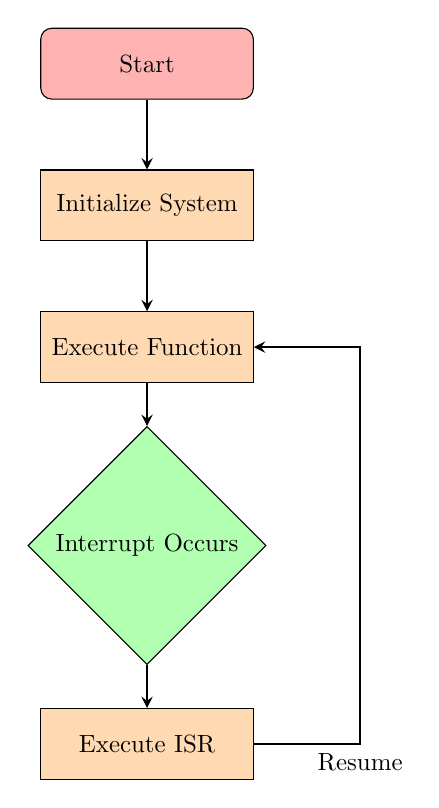
\begin{tikzpicture}[node distance=2cm, scale=0.9, transform shape]
				
				\node (start) [startstop] {Start};
				\node (init) [process, below of=start] {Initialize System};
				\node (exec) [process, below of=init] {Execute Function};
				\node (interrupt) [decision, below of=exec, yshift=-0.8cm] {Interrupt Occurs};
				\node (isr) [process, below of=interrupt, yshift=-0.8cm] {Execute ISR};
				
				\draw [arrow] (start) -- (init);
				\draw [arrow] (init) -- (exec);
				\draw [arrow] (exec) -- (interrupt);
				\draw [arrow] (interrupt) -- node[anchor=east] {} (isr);
				
				% Arrow from ISR to Execute Function with 'Resume' label below
				\draw [arrow] (isr.east) -- ++(1.5,0) |- (exec.east) node[pos=0,below] {Resume};
				
			\end{tikzpicture}
			\caption{Flowchart of the Interrupt-Driven System}
			\label{fig:ids}
		\end{figure}
		
		In Figure \ref{fig:ids}, a basic execution flow of a interrupt-driven system is displayed. The system executes a function as long as no interrupt occurs. When an interrupt occurs, it switches to the \ac{ISR}, executes it, and then resumes the function executed before the interrupt happened.
		
		The management of interrupts represents the most challenging aspect of an interrupt-driven system, as it is crucial to maintain the system's fast responsiveness. Interrupts occur in unpredictable ways, so you have to consider every possible execution flow. To ensure the execution of critical interrupts, interrupts are often prioritized, so higher-priority events can interrupt lower ones and be handled immediately. When handling an interrupt, the current state of the processor is saved, and the context is switched to the \ac{ISR} \cite{wang2020}.
		
		The unpredictability and asynchronous nature of interrupts present many challenges in an interrupt-driven system. One of the biggest challenges is the correct handling of the different priorities of the interrupts.\cite{wang2020}
		To conclude in an interrupt-driven system, the execution of the main program and \acp{ISR} needs to be handled properly to ensure data integrity. 
		
		\section{Shared Resources}
		Analyzing the management of shared resources is a large part of data race analysis, which is further explained later. The following is a short introduction to shared resources to better understand them in the context of data races.
		
		Shared resources, often referred to as shared memory or shared variables, are data that can be accessed simultaneously by multiple threads or processes. Proper management of these resources is crucial because improper handling can lead to issues like data races, deadlocks, and other synchronization problems. In interrupt-driven systems, shared resources often involve variables or data structures that are accessed by both the main program and \acp{ISR}. Proper management of shared resources is critical to ensure data consistency and avoiding conflicts \cite{herlihy2008}.
		
		Management of shared resources involves the use of synchronization mechanisms to coordinate access and ensure data consistency. Mutexes, semaphores, and condition variables are common tools used to control access to shared resources. Mutexes provide mutual exclusion, ensuring that only one thread can access the resource at a time. Semaphores can limit the number of threads accessing the resource simultaneously. Condition variables allow threads to wait for certain conditions to be met before proceeding, facilitating complex synchronization scenarios \cite{herlihy2008}. In interrupt-driven software, the synchronization of shared resources often involves disabling interrupts while accessing shared data \cite{chopra2019}.
		
		\section{Reduced Inter-Procedural Control Flow Graphs}
		Control flow graphs (\acs{CFG}) are representations of all possible paths through a program or function during its execution. An \acp{ICFG} adds possible edges between multiple programs or functions to also show possible control flows between those \cite{mehl2008}.\\
		An \acl{ICFG} is a directed graph $G = (V, E)$ where:
		\begin{itemize}
			\item $V$ is the set of vertices. Each vertex represents a \ac{BB} within a procedure or function.
			\item $E$ is the set of directed edges. Each edge $(u, v)$ represents a possible flow of control from block $u$ to block $v$. These edges include:
			\begin{itemize}
				\item Intra-procedural edges, which represent the control flow within a single function.
				\item Call edges, which represent the calling of a function \cite{mehl2008}.
			\end{itemize}
		\end{itemize}
		 An \ac{RICFG} is an optimized version of the \ac{ICFG} that simplifies the graph to only the necessary information needed for the analysis \cite{wang2020}.
		
		\begin{figure}[H]

			\centering
			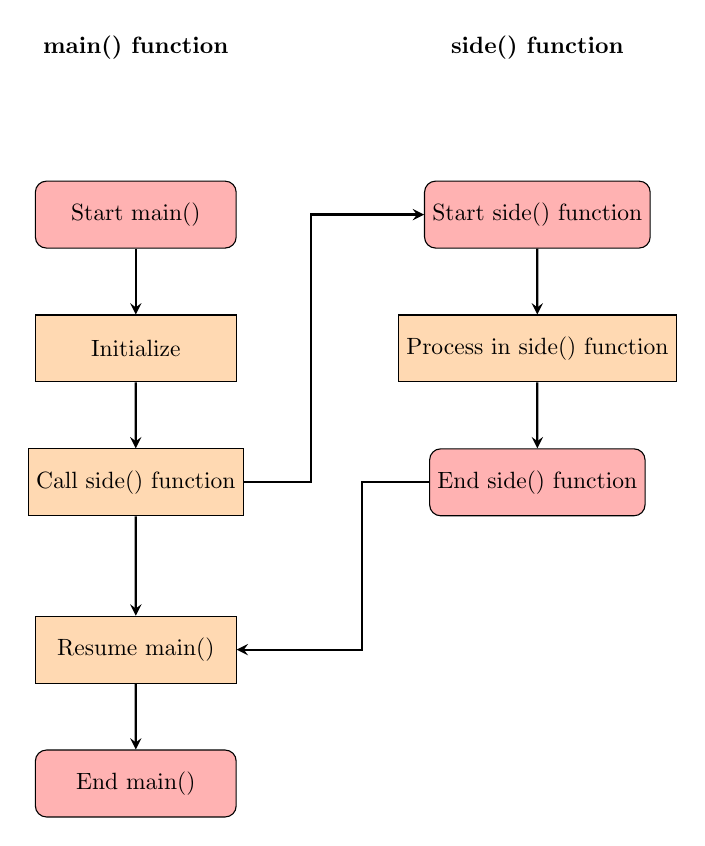
\begin{tikzpicture}[node distance=2cm, scale=0.85, transform shape]
				
				% Nodes for main function
				\node (start) [startstop] {Start main()};
				\node (init) [process, below of=start] {Initialize};
				\node (callsidefunction) [process, below of=init] {Call side() function};
				\node (resume) [process, below of=callsidefunction, yshift=-0.5cm] {Resume main()};
				\node (end) [startstop, below of=resume] {End main()};
				
				% Nodes for sidefunction
				\node (startsidefunction) [startstop, right of=callsidefunction, xshift=4cm, yshift=4cm] {Start side() function};
				\node (processsidefunction) [process, below of=startsidefunction] {Process in side() function};
				\node (endsidefunction) [startstop, below of=processsidefunction] {End side() function};
				
				% Arrows for main function
				\draw [arrow] (start) -- (init);
				\draw [arrow] (init) -- (callsidefunction);
				\draw [arrow] (callsidefunction) -- (resume);
				\draw [arrow] (resume) -- (end);
				
				% Arrows for sidefunction
				\draw [arrow] (startsidefunction) -- (processsidefunction);
				\draw [arrow] (processsidefunction) -- (endsidefunction);
				
				% Interprocedural arrows
				\draw [arrow] (callsidefunction.east) -- ++(1,0) |- (startsidefunction);
				\draw [arrow] (endsidefunction.west) -- ++(-1,0) |- (resume);
				
				% Labels
				\node [above of=start, yshift=0.5cm, text centered] {\textbf{main() function}};
				\node [above of=startsidefunction, yshift=0.5cm, xshift=0cm, text centered] {\textbf{side() function}};
				
			\end{tikzpicture}
			\caption{Example of an Inter-Procedural Control Flow Graph}
			\label{icfg}
		\end{figure}
		
		In Figure \ref{icfg}, a simple \ac{ICFG} is shown. There are two separate linear control flow graphs where the main function calls the side function in its execution. To interpret the flow of the program correctly, you need to consider the execution of sidefunction() and where it's called. The \ac{ICFG} combines the two separate CFGs to ensure correct analysis.
		
		\subsection{Reduction of Control Flow Graphs}
		There are multiple techniques to reduce the graph, without losing any information required for the analysis and reducing the complexity of the \ac{RICFG}. The reduction of the \ac{ICFG} makes the analysis of large and complex software a lot more efficient. By minimizing the amount of data while maintaining sufficient detail, \acp{RICFG} are a effective tool for the static analysis of data races \cite{gold2014}\cite{wang2020}.
		
		 The elimination of nodes is the main tool used in this work to reduce the CFG. Eliminating nodes that do not carry any essential information for the applied data analysis significantly reduces the amount of data the algorithm has to analyze. Overall, the reduction enhances the scalability of static analysis and make it more practical to analyze more complex data structures \cite{wang2020}.
		
		\begin{figure}[H]
			\centering
			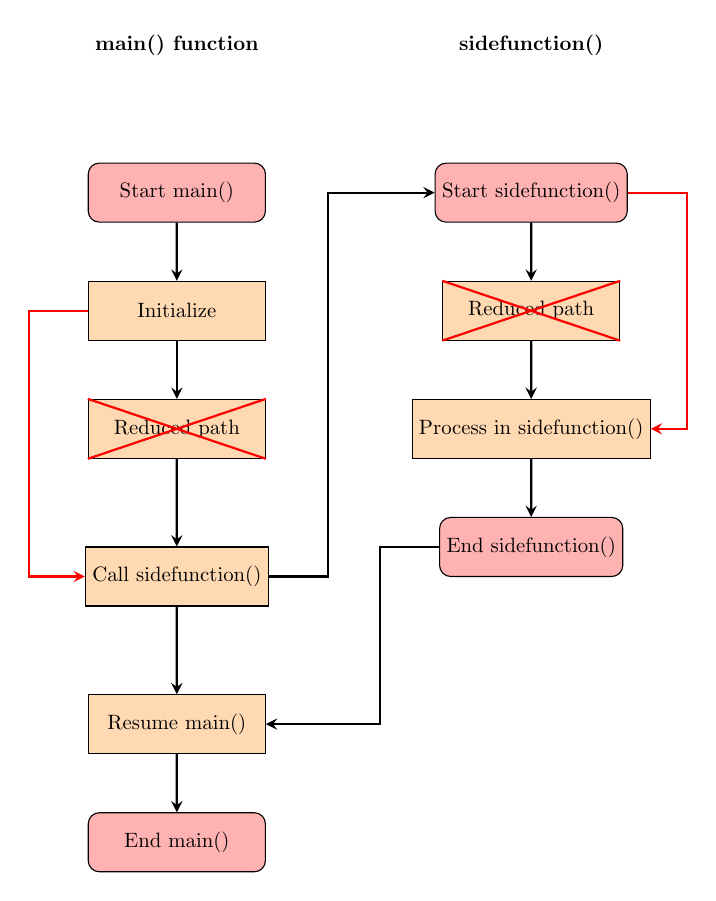
\begin{tikzpicture}[node distance=2cm, scale=0.75, transform shape]
				
				% Nodes for main function
				\node (start) [startstop] {Start main()};
				\node (init) [process, below of=start] {Initialize};
				\node (unimportant_main) [process, below of=init] {Reduced path};
				\node (callisr1) [process, below of=unimportant_main, yshift=-0.5cm] {Call sidefunction()};
				\node (resume) [process, below of=callisr1, yshift=-0.5cm] {Resume main()};
				\node (end) [startstop, below of=resume] {End main()};
				
				% Nodes for \ac{ISR}1 function
				\node (startisr1) [startstop, right of=callisr1, xshift=4cm, yshift=6.5cm] {Start sidefunction()};
				\node (unimportant_isr1) [process, below of=startisr1] {Reduced path};
				\node (processisr1) [process, below of=unimportant_isr1] {Process in sidefunction()};
				\node (endisr1) [startstop, below of=processisr1] {End sidefunction()};
				
				% Arrows for main function
				\draw [arrow] (start) -- (init);
				\draw [arrow] (init) -- (unimportant_main);
				\draw [arrow] (unimportant_main) -- (callisr1);
				\draw [arrow] (callisr1) -- (resume);
				\draw [arrow] (resume) -- (end);
				
				% Arrows for \ac{ISR}1 function
				\draw [arrow] (startisr1) -- (unimportant_isr1);
				\draw [arrow] (unimportant_isr1) -- (processisr1);
				\draw [arrow] (processisr1) -- (endisr1);
				
				% Interprocedural arrows
				\draw [arrow] (callisr1.east) -- ++(1,0) |- (startisr1);
				\draw [arrow] (endisr1.west) -- ++(-1,0) |- (resume);
				
				% Red arrows bypassing unimportant information
				\draw [redarrow] (init.west) -- ++(-1,0) |- (callisr1.west);
				\draw [redarrow] (startisr1.east) -- ++(1,0) |- (processisr1.east);
				
				% Red crosses over unimportant information
				\draw[red,thick] (unimportant_main.north west) -- (unimportant_main.south east);
				\draw[red,thick] (unimportant_main.north east) -- (unimportant_main.south west);
				\draw[red,thick] (unimportant_isr1.north west) -- (unimportant_isr1.south east);
				\draw[red,thick] (unimportant_isr1.north east) -- (unimportant_isr1.south west);
				
				% Labels
				\node [above of=start, yshift=0.5cm, text centered] {\textbf{main() function}};
				\node [above of=startisr1, yshift=0.5cm, xshift=0cm, text centered] {\textbf{sidefunction()}};
				
			\end{tikzpicture}
			\caption{Example of a Reduced Inter-Procedural Control Flow Graph}
			\label{ricfg}
		\end{figure}
		
		Figure \ref{ricfg} shows the example of a simple \ac{ICFG} with added unneccessary nodes. The resulting \ac{RICFG} reduces the \ac{CFG} by eliminating the nodes that do not carry any important information for the analysis the \ac{RICFG} is used for. It also adds new edges to skip the deleted nodes.
		 
		\subsection{Depth-First Search}
		\ac{DFS} is an algorithm used to traverse a graph systematically. It begins at a source node and extends its exploration through the connected nodes as far as possible before it backtracks. In an algorithm this can be implemented using a recursive approach. The basic idea is to mark a node when its first discovered and then explore all the adjacent nodes that are not visited before. 
		
		\begin{algorithm}[H]
			\label{algo:dfs}
			\caption{Depth-First Search}
			\SetAlgoLined
			\SetKwFunction{FMain}{dfs\_main}
			\SetKwFunction{DFS}{dfs}
			\SetKwProg{Fn}{Function}{:}{}
			
			\Fn{\DFS{node, visited}}{
				visited[node] = True\;
				\For{neighbor \textbf{in} graph[node]}{
					\If{not visited[neighbor]}{
						\DFS{neighbor, visited}\;
					}
				}
			}
		\end{algorithm}
		
		Algorithm \ref{algo:dfs} shows the algorithm that is used to execute an \ac{DFS}. The \texttt{dfs} function gets called with the root node of a tree and performs the \ac{DFS} starting from the given node. It recursively calls itself with a new node called \texttt{neighbor} and repeats this until all the reachable nodes are marked as visited \cite{mehl2008}.
		\begin{figure}[H]
			
		\centering
		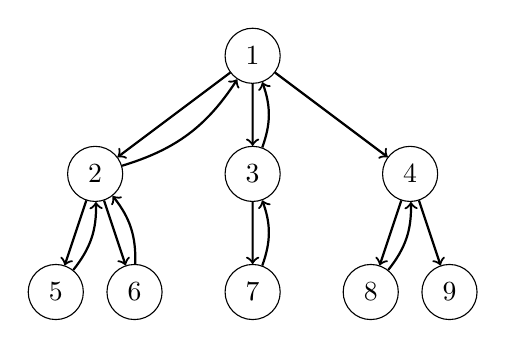
\begin{tikzpicture}[
			every node/.style={circle, draw, minimum size=7mm},
			level/.style={sibling distance=20mm/#1}
			]
			
			% Tree nodes
			\node (1) {1}
			child {node (2) {2}
				child {node (5) {5}}
				child {node (6) {6}}
			}
			child {node (3) {3}
				child {node (7) {7}}
			}
			child {node (4) {4}
				child {node (8) {8}}
				child {node (9) {9}}
			};
			
			% DFS traversal edges with smaller backtracking arrows
			\draw[->, thick] (1) -- (2);
			\draw[->, thick] (2) -- (5);
			\draw[->, thick] (5) edge[bend right=20, ->, thick] (2); % Smaller backtrack arrow from 5 to 2
			\draw[->, thick] (2) -- (6);
			\draw[->, thick] (6) edge[bend right=20, ->, thick] (2); % Smaller backtrack arrow from 6 to 2
			\draw[->, thick] (2) edge[bend right=20, ->, thick] (1); % Smaller backtrack arrow from 2 to 3
			\draw[->, thick] (1) -- (3);
			\draw[->, thick] (3) -- (7);
			\draw[->, thick] (7) edge[bend right=20, ->, thick] (3); % Smaller backtrack arrow from 7 to 3
			\draw[->, thick] (3) edge[bend right=20, ->, thick] (1); % Smaller backtrack arrow from 3 to 4
			\draw[->, thick] (1) -- (4);
			\draw[->, thick] (4) -- (8);
			\draw[->, thick] (8) edge[bend right=20, ->, thick] (4); % Smaller backtrack arrow from 8 to 4
			\draw[->, thick] (4) -- (9);
			
		\end{tikzpicture}
		\caption{Depth-First Search of a Tree}
		\label{dfstree}
		\end{figure}
		Figure \ref{dfstree} displays the execution of a \ac{DFS}. Starting from node 1 the algorithm goes to the next node here node 2. From there it traverses to the next node in line, which is linked with node 2. Node 5 is the end of the branch and has no successors. From a node like this the algorithm backtracks to the last node that had a successor, here shown with a curved arrow. This process repeats through the whole tree resulting in the traversion of the tree in the following order: 1,2,5,6,3,7,4,8,9.
		\section{Data Races}
		
		A data race occurs when two or more functions or threads access a shared resource concurrently, without being ordered by a happens-before relationship, and one of those accesses is a write operation \cite{chen2011}. A happens-before relationship ensures that, if there are two operations A and B and they are related in a happens-before relationship A has to finish before B can start. Data races can lead to unpredictable behavior and errors in the system, which makes the detection of data races a critical aspect of concurrent programs. Without proper synchronization, a system with multiple threads or functions that use shared data may lead to data races. The outcome of a interrupt-driven program with data races is non-deterministic. The order of execution of operations vary, which may result in bugs that are not reproducible or difficult to reproduce \cite{chen2011}.
		
		\begin{figure}[H]
			\begin{lstlisting}
				# Data Race Example
				long shared1 = 0
				
				def main():
				
				unsigned tmp = 0
				
				tmp = shared1
				
				def isr1():
				
				idlerun()
				shared1 = 1
				idlerun()
				
				main()
			\end{lstlisting}
			\caption{Simple Data Race Example}
			\label{raceexample}
		\end{figure}	
		
		Figure \ref{raceexample} shows a simple example of a possible data race between a \texttt{main} function and an \texttt{isr} function. A global variable \texttt{shared1} is initiated and accessed in two different functions, \texttt{main()} and \texttt{isr1()}. Since there are no synchronization tools used and the operation in \texttt{isr1} is a write, there is a data race between line 5 and line 9.
		
		\subsection{Detection Techniques}
		
		Data race detection can be approached by two different analytical methods. Each of these methods provides benefits and challenges.
		
		\subsubsection{Static Data Race Detection}
		Static data race detection involves analyzing the source code of a program without executing it to identify potential race conditions, which are situations where the outcome of a program depends on the timing of uncontrollable events like thread execution order \cite{wang2020}. \\
		\textbf{Advantages:}
		\begin{itemize}
			\item Comprehensiveness: Static analysis inspects the code without executing the program by analyzing every possible execution path and interaction that could lead to data races \cite{wang2020}.
			\item Early Detection: Since static analysis does not require execution, it can analyze the code in the development phase, allowing the developer to find issues without deployment \cite{chen2011}.
		\end{itemize}
		\textbf{Disadvantages:}
		\begin{itemize}
			\item False Positives/Negatives: Static analysis reports all data races that fall under certain conditions. Some of these data races could be very unlikely or even impossible at runtime. On the other hand, due to the approximations and assumptions necessary for tractability, it may miss some races \cite{chen2011}.
			\item Complexity in Handling Dynamic Behavior: Dynamic behaviors such as pointers or recursion can be challenging to analyze for static approaches, leading to incomplete or inaccurate results \cite{wang2020}.
		\end{itemize}
		
		\subsubsection{Dynamic Data Race Detection}
		Dynamic data race detection, on the other hand, involves monitoring the execution of a program in real-time to detect actual race conditions as they occur, relying on runtime information to identify conflicts in memory access by concurrent threads \cite{engler2003}. \\
		\textbf{Advantages:}
		\begin{itemize}
			\item Precision: Dynamic analysis tools monitor the actual execution of a program, identifying data races in real-time, which reduces the number of false positives \cite{engler2003}.
			\item Context-Sensitive Detection: By analyzing the actual runtime behavior, dynamic analysis can understand the context of operations, leading to more accurate detection \cite{engler2003}.
		\end{itemize}
		\textbf{Disadvantages:}
		\begin{itemize}
			\item Performance Overhead: The analysis at runtime can slow down the application significantly \cite{chen2011}.
			\item Coverage: The effectiveness is heavily dependent on the execution path triggered during the tests. If certain parts of the program are not passed through in the execution run, they are not analyzed \cite{engler2003}.
		\end{itemize}
		
		Both static and dynamic analyses are crucial for a complete analysis of code. They complement each other's limitations. A combination of both is the best approach to detect data races most reliably.\cite{engler2003} However, this work, focuses on the static analysis of data races.
		
		\subsection{Strategies for Preventing Data Races}
		
		Preventing data races requires careful design and implementation of concurrent programs. Effective strategies for general prevention of data races are synchronization mechanisms such as mutexes, semaphores, and condition variables, which control access to shared data. These mechanisms ensure that only one thread can access the shared resource at a time \cite{herlihy2008}. Since this work focuses on data races in interrupt-driven systems, the main tool to prevent data races is to disable \acp{ISR}, which access shared resources in critical areas. The correct analyzation of those synchronization mechanisms prevents false posititves.
		\begin{figure}[H]
		
			\begin{lstlisting}
				# Data Race Example with ISR Enable/Disable
				long shared1 = 0;
				
				def main():
				
				unsigned tmp = 0;
				disable_isr(1);
				tmp = shared1;
				enable_isr(1);
				def isr1():
				
				idlerun();
				shared1 = 1;
				idlerun();
				
				main();
			\end{lstlisting}
			\caption{Data Race Example with ISR Enable/Disable}
			\label{drisr}
		\end{figure}
		Figure \ref{drisr} shows an example for a disable and enable call that lead to the safe access of shared data. The \texttt{main()} function and \texttt{isr1()} both access the shared resource \texttt{shared1}. Since the read operation in line 6 of the \texttt{main()} function is safely accessed by disabling \texttt{isr1} in line 5 and enabling it in line 7, a possible data race is prevented.
		
		\section{Static Detection of Data Races in Interrupt-Driven Systems}
		
		The asynchronous nature and concurrent execution of \acp{ISR} and the main function introduce significant challenges for data consistency and detecting data races in interrupt-driven systems. Static data race analyses, especially those who utalize \acp{RICFG}, are a promising approach to identify data races without the need for extensive testing and runtime monitoring as in dynamic approaches \cite{wang2020}.
		
		The static approach involves the construction of an \ac{RICFG} for the program, which includes both the main code and \acp{ISR}, and capturing the control flow and potential interaction between them. Traversion of the \ac{RICFG} using a \Ac{DFS} shows paths where shared resources are accessed concurrently without proper synchronization and indicates potential data races. Integrating the static analysis tool with the development process enables continuous detection of data races during software development, which improves the reliability and correctness of interrupt-driven systems \cite{wang2020}.
		
		The methodology for static data race detection in interrupt-driven systems by Wang et al. \cite{wang2020} involves the following key steps.
		\begin{enumerate}
			\item First, the \acp{RICFG} are constructed for the entire program, including the main code and the \acp{ISR}. This involves analyzing the control flow and identifying interactions between the main program and \acp{ISR}. 
			\item Next, the \acp{RICFG} are analyzed to find potential data races, focusing on paths where concurrent access to shared data is done without proper synchronization. 
			\item Finally, the developer can use the analysis results to address identified data races early in the development process \cite{wang2020}.
		\end{enumerate}
		
		\begin{algorithm}[H]
			\label{algo:srd}
			\caption{Static Race Detection}
			\KwIn{RICFGs of P}
			\KwOut{potential racing pairs (PR)}
			
			\BlankLine
			\For{each $< G_i ; G_j >$ in RICFGs}{
				\For{each $sv_i \in G_i$}{
					\For{each $sv_j \in G_j$}{
						\If{$sv_i.V == sv_j.V$ and $(sv_i.A == W$ or $sv_j.A == W)$ and $G_i.pri < G_j.pri$ and $INTB.get(svi).contains(Gj)$}{
							$PR = PR \cup \{ <sv_i, sv_j> \}$\;
						}
					}
				}
			}
		\end{algorithm}
		
		The \textit{Static Race Detection} algorithm by Wang et al. \cite{wang2020}, presented in Algorithm \ref{algo:srd} , takes the \acp{RICFG} of program $P$ as input and outputs the potential racing pairs (PR). For each pair of graphs $< G_i ; G_j >$ in the \acp{RICFG}, the algorithm iterates over each shared variable $sv_i$ in $G_i$ and each shared variable $sv_j$ in $G_j$. If the variables $sv_i$ and $sv_j$ are the same ($sv_i.V == sv_j.V$), at least one of the accesses is a write operation ($(sv_i.A == W$ or $sv_j.A == W)$), the priority of $G_i$ is less than that of $G_j$ ($G_i.pri < G_j.pri$), and the interrupt status table ($INTB$) indicates that the interrupt for $sv_i$ is enabled while $sv_j$ is being accessed, then the pair $<sv_i, sv_j>$ is added to the set of potential racing pairs (PR) \cite{wang2020}.
		
		The following chapter introduces the implementation of a new static analysis program based on the static race detection approach of Wang et al. \cite{wang2020}.
	
	\section{\acl{GCC}}
		For the generation of the input, \ac{GCC}\footnote{\href{https://gcc.gnu.org/}{https://gcc.gnu.org/}} is used. \Ac{GCC} is a suite for compilers for various programming languages, including C and C++, among others. The command \texttt{gcc -fdump-tree-cfg} generates a \mbox{\texttt{cfg-file}} out of a program file, with all the important information for the intended data race analysis.
		\begin{figure}[H]
			\begin{adjustbox}{scale=1}
				\begin{lstlisting}
					;; Function int main()
					
					;;  nodes: 0 1 2 3 4 5 6
					;; 2 succs { 3 4 }
					;; 3 succs { 5 }
					;; 4 succs { 5 }
					;; 5 succs { 6 }
					;; 6 succs { 1 } 
					
					int main() ()
					{
						int variable2;
						unsigned char tmp;
						int D.1934;
						long int shared1.2;
						long int shared1.1;
						bool retval.0;
						
						<bb 2>:
						disable_isr (1);
						shared1 = 0;
						shared1.1 = shared1;
						retval.0 = shared1.1 != 0;
						if (retval.0 != 0)
						goto <bb 3>;
						else
						goto <bb 4>;
						
						<bb 3>:
						enable_isr (1);
						goto <bb 5>;
						
						<bb 4>:
						variable2 = 1;
						
						<bb 5>:
						shared1.2 = shared1;
						tmp = (unsigned char) shared1.2;
						enable_isr (1);
						D.1934 = 0;
						
						<L3>:
						return D.1934;
					}
				\end{lstlisting}
			\end{adjustbox}
			\caption{Example CFG generated with GCC}
			\label{fig:gcc}
		\end{figure}
		Figure \ref{fig:gcc} shows an reduced example of a \texttt{cfg-file} generated with \ac{GCC}, which displays the later used parts of the \texttt{cfg-file}.
		In line 1 of each \texttt{cfg-file} is a commented line with the function name. This line is used to strip the function name in the implementation.
		
		Following the function name, in line 3 to 8, there is summary of every \acl{BB} including their successors. This part is used to add the successors of each \aclp{BB} to their initiated items. 
		
		Finally there is the actual execution of each function in line 10 to 44. It displays each \acl{BB} and what they do. This part is used to find critical lines that access the shared resource or changing the status of an \ac{ISR}.


\chapter{Implementation}
The following chapter provides an in-depth explanation of the implementation. 
\begin{figure}[H]
	\centering
	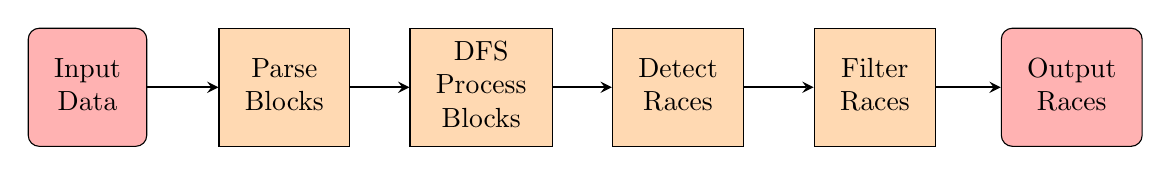
\begin{tikzpicture}[node distance=2.5cm]
		
		% Define styles only within this scope
		\begin{scope}[
			startstop/.style={rectangle, rounded corners, minimum width=1.5cm, minimum height=1.5cm, text centered, draw=black, fill=red!30},
			process/.style={rectangle, minimum width=1.5cm, minimum height=1.5cm, text centered, draw=black, fill=orange!30},
			arrow/.style={thick,->,>=stealth}
			]
			
			\node (start) [startstop] {\begin{tabular}{c}Input\\Data\end{tabular}};
			\node (parse) [process, right of=start] {\begin{tabular}{c}Parse\\Blocks\end{tabular}};
			\node (dfs) [process, right of=parse] {\begin{tabular}{c}DFS\\Process\\Blocks\end{tabular}};
			\node (detect) [process, right of=dfs] {\begin{tabular}{c}Detect\\Races\end{tabular}};
			\node (filter) [process, right of=detect] {\begin{tabular}{c}Filter\\Races\end{tabular}};
			\node (output) [startstop, right of=filter] {\begin{tabular}{c}Output\\Races\end{tabular}};
			
			\draw [arrow] (start) -- (parse);
			\draw [arrow] (parse) -- (dfs);
			\draw [arrow] (dfs) -- (detect);
			\draw [arrow] (detect) -- (filter);
			\draw [arrow] (filter) -- (output);
			
		\end{scope}
	\end{tikzpicture}
	\caption{Flow Chart of the Program}
	\label{programflowchart}
\end{figure}
Figure \ref{programflowchart} shows the flow of the data race analysis. First the input is parsed and generates the \aclp{BB} items, which are then traversed using a \ac{DFS} and processed while traversing through them. With the information generated by the traversion of the \ac{RICFG} possible data races are detected and saved. Finally correct shared data accesses that meet the criterias used in the data race detection are filtered out of the list of data races.
The explanation of the implementation is split into the initialization of the basic block class, the parsing of the input, the \acl{DFS} to explore all path, the actual data race analysis, and the filtering of false positives found in the data race analysis.


\section{Class BasicBlock}

The class \texttt{BasicBlock} displays all the information necessary for the data race analysis. The \aclp{BB} build the \ac{RICFG} by storing every possible path of the functions in its successors. Each \ac{BB} item also stores all the important informations for the further data race analysis like priority of the function, shared resource access in the \ac{BB}, enable or disable calls of \acp{ISR} and function calls for inter-procedural edges between the function. Those information include the following attributes:
\begin{itemize}
	\item \texttt{function\_name}: The function name to which the basic block belongs.
	\item \texttt{number}: The number of the basic block.
	\item \texttt{priority}: The priority of the function the \ac{BB} is in.
	\item \texttt{shared\_resources}: All accesses of shared resources within the \ac{BB}. The access type (read/write) and the line number of such calls are saved.
	\item \texttt{successors}: A list of all the successors of each basic block. Important for building all possible paths through the CFG.
	\item \texttt{enable\_disable\_calls}: All calls that disable or enable an \ac{ISR} within this basic block and also the corresponding line number of those calls to ensure the correct order.
	\item \texttt{function\_calls}: The functions that are called within a \ac{BB}.
\end{itemize}
To summarize, Figure \ref{uml} shows the UML diagram of the \texttt{BasicBlock} class.
\begin{figure}[H]
	\centering
	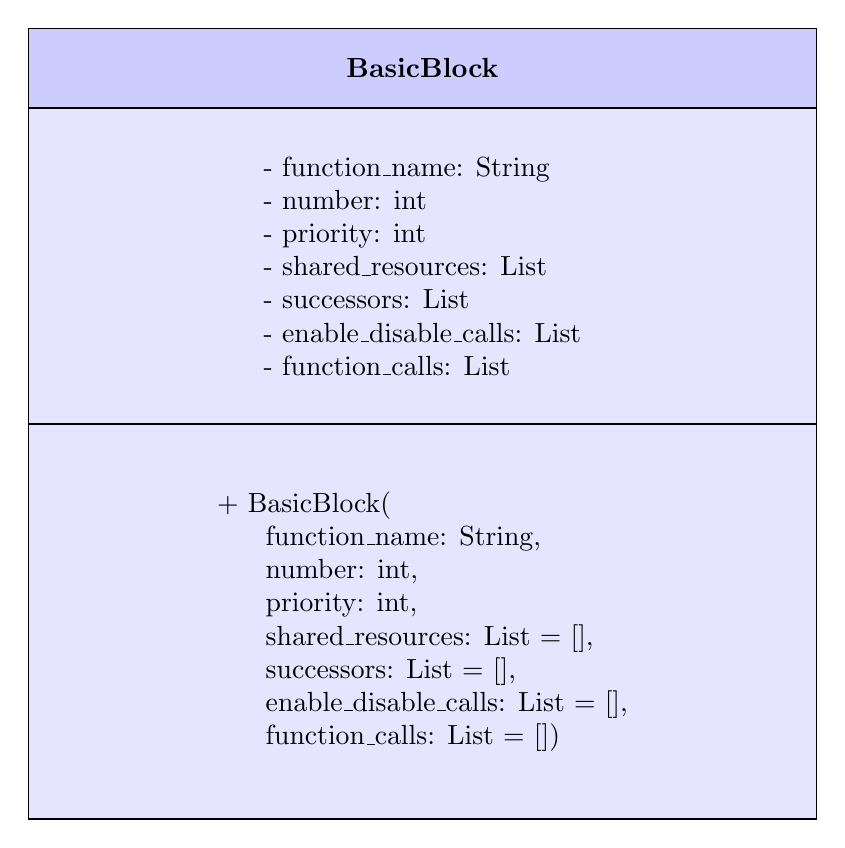
\begin{tikzpicture}
		% Define styles for the different elements of the class diagram
		\tikzstyle{class} = [rectangle, draw, minimum width=10cm, minimum height=1cm, font=\bfseries, fill=blue!20]
		\tikzstyle{attributes} = [rectangle, draw, minimum width=10cm, minimum height=4cm, anchor=north, align=left, fill=blue!10]
		\tikzstyle{methods} = [rectangle, draw, minimum width=10cm, minimum height=5cm, anchor=north, align=left, fill=blue!10]
		
		% Class name
		\node[class] (classname) at (0, 0) {BasicBlock};
		
		% Attributes
		\node[attributes, below=0cm of classname] (attributes) {
			- function\_name: String\\
			- number: int\\
			- priority: int\\
			- shared\_resources: List\\
			- successors: List\\
			- enable\_disable\_calls: List\\
			- function\_calls: List
		};
		
		% Methods
		\node[methods, below=0cm of attributes] (methods) {
			+ BasicBlock(\\
			\hspace*{5mm} function\_name: String,\\
			\hspace*{5mm} number: int,\\
			\hspace*{5mm} priority: int,\\
			\hspace*{5mm} shared\_resources: List = [],\\
			\hspace*{5mm} successors: List = [],\\
			\hspace*{5mm} enable\_disable\_calls: List = [],\\
			\hspace*{5mm} function\_calls: List = [])
		};
		
		% Draw the borders
		\draw (classname.north west) rectangle (methods.south east);
		\draw (attributes.north west) -- (attributes.north east);
		\draw (methods.north west) -- (methods.north east);
	\end{tikzpicture}
	\caption{UML: Class BasicBlock}
	\label{uml}
\end{figure}

\section{Parsing and Helper Functions}
This section explains the parsing of the input and the helper functions, which are called in the data race analysis.

The parsing of the input iterates two times through the code lines to extract all the important information of the code and save it in the \ac{BB} items. The first iteration of the code lines initiates the \acp{BB} with the \ac{BB} number and the function it relates to.
Using these regular expression:
\begin{lstlisting}
	func_match = re.match(r';; Function (.+?) \(', line)
	bb_match = re.match(r'<bb (\d+)>:', line)
\end{lstlisting}
Additionally, it adds the information of shared resources, enable/disable calls of \acp{ISR} and function calls within the \ac{BB}.
To identify the shared reources and their operation type these regular expression are used:
\begin{lstlisting}
	re.search(fr'\b{resource_name}\b', line)
	re.search(fr'\b{resource_name}\b\s*=', line) and not re.search(fr'\b{resource_name}\b\s*==', line)
\end{lstlisting}
The second iteration adds the successors of the \ac{BB}, using this regular expression:
\begin{lstlisting}
	succ_match = re.match(r';; (\d+) succs \{(.+?)\}', line)
\end{lstlisting}
A second iteration is used to ensure all the \acp{BB} items are initialized first to ensure a correct handling of the successors.

There are also multiple helper functions, which are called during the data race analysis part of the implementation. 

The \texttt{determine\_priority} function is determining the priority of the function which is involved in a possible data race. Since one condition for a data race is that the interrupting function has a higher priority, this is an important check. The function uses a regular expression to find the number of a \ac{ISR} to use that as its priority.
\begin{lstlisting}
	match = re.search(r'isr[_]?(\d+)', function_name)
\end{lstlisting}
The priority is determined in the first place by differentiating between \ac{ISR} functions and normal functions because \acp{ISR} always have a higher priority than non-\ac{ISR} functions. In this implementation non-\Ac{ISR} functions have the priority infinity and \acp{ISR} are ordered by the number of it, while lower number \acp{ISR} have a higher priority than higher number ones.
	
The \texttt{propagate\_function\_calls} function is handling the case of a function that calls another function. It checks for \acp{BB} items with a function call in it and adds the critical parts of the called function to the current \ac{BB} to simulate a path through the called function and consider the shared resources and enable/disable calls of that function.

\section{Data Race Detection}
The following algorithms are used to determine all possible data races, which are filtered later in the code. The intention is to find all possible data races to minimize the number of false negatives, since false positives can be evaluated later by interpreting the output.

 The algorithms are ordered as they are found in the code. All the following algorithms are part of the \texttt{detect\_data\_race} function in the program. The \ac{DFS} algorithm is exploring all possible paths thorugh the \ac{CFG} while calling the Algorithm \ref{algo:PB} Process Block, which processes the shared resources and enable or disable calls within the \ac{BB} in order. It appends the shared resources to a list \texttt{resource\_access} and updates the \texttt{current\_isr\_status}. The resource access list is then used in the Alogrithm \ref{checkdr} Check for Data Races, where it finds possible data races using the critical criterias of a data race. In the end the Algorithm \ref{filterdr} Filter Data Races is using the \texttt{isr\_status} aswell as the \texttt{isr\_enabling\_map} to filter out correctly accessed shared resources.

The first part of the function \texttt{detect\_data\_races} takes a list of all basic block items as input. It also initializes the empty list \texttt{potential\_data\_races}, a dictionary for \texttt{resource\_access}, and a dictionary for the \texttt{isr\_enabling\_map}. \texttt{Potential\_data\_races} and \texttt{resource\_access} are used later in the code.

\begin{algorithm}[H]
	\caption{ISR Enabling Map}
	\label{algo:isrmap}
	\DontPrintSemicolon
	\SetAlgoLined
	\KwData{blocks}
	\KwResult{List ISR enabling ISRs filled}
	\SetKwInOut{Input}{input}\SetKwInOut{Output}{output}
	\KwIn{Dictionary of BasicBlocks}
	\KwOut{List of enabling ISRs}
	\BlankLine
	isr\_enabling\_map $\gets$ initialize as a default dictionary to set\;
	\BlankLine
	\ForEach{block in blocks}{
		\ForEach{call, line\_number in block.enable\_disable\_calls}{
			\If{call contains 'enable\_isr'}{
				isr\_idx\_match $\gets$ search for isr number in call;\\
				\If{isr\_idx\_match is found}{
					enabled\_isr\_idx $\gets$ integer value of the first group in isr\_idx\_match minus one\;
					enabler\_isr $\gets$ block.function\_name\;
					isr\_enabling\_map[enabler\_isr].add(enabled\_isr\_idx)\;
				}
			}
		}
	}
\end{algorithm}

\vspace{1cm}
The main loop of the Algorithm \ref{algo:isrmap} iterates through every item in blocks and finds basic blocks with \texttt{enable\_disable\_calls}. If there is an enable call in a block item, the index of the enabled \ac{ISR} is read, and the basic block is added to the \texttt{isr\_enabling\_map} with the information of which \ac{ISR} it enables.

\begin{algorithm}[H]
	\caption{Process Block}
	\label{algo:PB}
	\DontPrintSemicolon
	\SetAlgoLined
	\KwData{block, current\_isr\_status}
	\KwResult{Updated ISR status and recorded resource accesses}
	\SetKwInOut{Input}{input}\SetKwInOut{Output}{output}
	\KwIn{A code block and the current ISR status as a list}
	\KwOut{Updated current ISR status and appended resource accesses to a global list}
	\BlankLine
	combined\_events $\gets$ sort(block.shared\_resources + block.enable\_disable\_calls, key=\texttt{lambda} x: x[2] if len(x) == 3 else x[1])\;
	\ForEach{event in combined\_events}{
		\If{event is a shared resource access (\texttt{len(event) == 3})}{
			resource\_name, access\_type, res\_line\_number $\gets$ event\;
			resource\_accesses[resource\_name].append((block.function\_name, block.number, access\_type, res\_line\_number, current\_isr\_status.copy(), block.priority))\;
		}
		\ElseIf{event is an enable/disable ISR call (\texttt{len(event) == 2})}{
			call, line\_number $\gets$ event\;
			isr\_idx\_match $\gets$ search for ISR number in call\;
			\If{isr\_idx\_match is found}{
				isr\_idx $\gets$ integer value of the first group in isr\_idx\_match minus one\;
				\eIf{"disable\_isr" is in call}{
					\If{0 $\leq$ isr\_idx $<$ length of current\_isr\_status}{
						current\_isr\_status[isr\_idx] $\gets$ 1\;  % Assuming 1 indicates disabled
					}
				}{
					\If{0 $\leq$ isr\_idx $<$ length of current\_isr\_status}{
						current\_isr\_status[isr\_idx] $\gets$ 0\;  % Assuming 0 indicates enabled
					}
				}
			}
		}
	}
\end{algorithm}
\vspace{1cm}

Algorithm \ref{algo:PB} iterates through each shared resource access and enable/disable call of a basic block to find the current \ac{ISR} status while resources are accessed. It sorts each access of shared resources and the enable or disable calls of \acp{ISR} by line number to ensure the correct order of execution. The algorithm differs between shared resource access and \Ac{ISR} enable or disable calls by the length of the event. Accesses have three entries, the resource name, the access type and the line number. The enable and disable calls have two entries the call and the line number. When a resource is found, all the information is added to the \texttt{resource\_accesses} dictionary, which includes the function name and the block number of the current basic block, as well as the access type, the line number, and the \ac{ISR} status of the access. If an enable or disable call is found the algorithm changes the corresponding bit in the \texttt{current\_isr\_status} array to 1 for diable calls and to 0 for enable calls. All this information is used later for the detection and filter of data races.

\begin{algorithm}[H]
	\caption{DFS and Initialization}
	\label{algo:dfs+init}
	\DontPrintSemicolon
	\SetAlgoLined
	\KwData{blocks}
	\KwResult{Updated block ISR statuses and processed blocks}
	\SetKwInOut{Input}{input}\SetKwInOut{Output}{output}
	\KwIn{Dictionary of basic blocks}
	\KwOut{Updated block ISR statuses}
	\BlankLine
	
	\SetKwProg{Fn}{Function}{:}{}
	\Fn{dfs(block, visited\_blocks, current\_isr\_status, path)}{
		\If{(block.function\_name, block.number) \textbf{in} visited\_blocks}{
			block\_isr\_statuses[(block.function\_name, block.number)] $\gets$ merge\_isr\_statuses(block\_isr\_statuses[(block.function\_name, block.number)], current\_isr\_status)\;
			\Return\;
		}
		visited\_blocks.add((block.function\_name, block.number))\;
		path.append((block.function\_name, block.number))\;
		
		block\_isr\_statuses[(block.function\_name, block.number)] $\gets$ current\_isr\_status.copy()\;
		process\_block(block, current\_isr\_status)\;
		
		\If{not block.successors}{
			\Return\;
		}
		\Else{
			\For{successor \textbf{in} block.successors}{
				dfs(successor, set(visited\_blocks), current\_isr\_status.copy(), path.copy())\;
			}
		}
	}
	
	\BlankLine
	\tcp{Initialization and starting DFS from basic blocks with number 2}
	\For{(func\_name, bb\_num), block \textbf{in} blocks.items()}{
		\If{bb\_num == 2}{
			initial\_isr\_status $\gets$ track\_isr\_status(blocks).copy()\;
			process\_block(block, initial\_isr\_status)\;
			\For{successor \textbf{in} block.successors}{
				dfs(successor, set(), initial\_isr\_status.copy(), [(func\_name, bb\_num)])\;
			}
		}
	}
\end{algorithm}
\vspace{1cm}
\begin{algorithm}[H]
	\label{Mergeisr}
	\caption{Merge ISR Statuses}
	\DontPrintSemicolon
	\SetAlgoLined
	\KwData{isr\_status1, isr\_status2}
	\KwResult{Merged ISR status list}
	\SetKwInOut{Input}{input}\SetKwInOut{Output}{output}
	\KwIn{Two lists of ISR statuses}
	\KwOut{List of merged ISR statuses}
	\BlankLine
	merged\_status $\gets$ empty list\;
	\For{isr1, isr2 \textbf{in} zip(isr\_status1, isr\_status2)}{
		merged\_status.append(min(isr1, isr2))\;
	}
	\Return{merged\_status}\;
\end{algorithm}

The Algorithm \ref{algo:dfs+init} is recursively traversing each block in a possible path of the \ac{RICFG}, while calling the \texttt{process\_block} function. The set \texttt{visited\_blocks} is used to avoid revisiting already visited blocks. If the block is already visited, the \ac{ISR} status is updated with the stored \ac{ISR} status for that block using the \texttt{merge\_isr\_statuses} function, shown in Algorithm \ref{Mergeisr}. It takes the worst case of the most enabled \acp{ISR} and uses this for further analysis of the path. 

Unvisited blocks get added to the \texttt{visited\_blocks} set and to the path list. After that, the \ac{ISR} status gets updated to the current \ac{ISR} status, and the function \texttt{process\_block} is called to update the \ac{ISR} status and track the shared resource accesses.

When the block is processed, the function checks for possible successors and recursively calls itself with the successor and the updated copy of \texttt{visited\_blocks}, \texttt{current\_isr\_status}, and the path.

The first \ac{BB} in a function is always the \ac{BB} with number two in the generated cfg-files. To initialize the \ac{DFS}, the \ac{BB} number 2 is processed by the \texttt{process\_block} function, and after that, the \ac{DFS} function is called with the successor of the current block.



\begin{algorithm}[H]
	\label{checkdr}
	\caption{Check for Data Races}
	\DontPrintSemicolon
	\SetAlgoLined
	\KwData{resource\_accesses}
	\KwResult{List of potential data races}
	\SetKwInOut{Input}{input}\SetKwInOut{Output}{output}
	\KwIn{Dictionary of resource accesses}
	\KwOut{List of potential data races}
	\BlankLine
	\SetKwFunction{FMain}{check\_for\_data\_races}
	\SetKwProg{Fn}{Function}{:}{}
	\Fn{\FMain{}}{
		\For{resource, accesses \textbf{in} resource\_accesses.items()}{
			\For{i, (func1, bb\_num1, access\_type1, line\_number1, isr\_status1, priority1) \textbf{in} enumerate(accesses)}{
				\For{j, (func2, bb\_num2, access\_type2, line\_number2, isr\_status2, priority2) \textbf{in} enumerate(accesses)}{
					\If{i $\geq$ j}{
						Continue\;
					}
					\If{func1 $\neq$ func2 \textbf{and} (access\_type1 == "write" \textbf{or} access\_type2 == "write") \textbf{and} priority1 $\neq$ priority2}{
						potential\_data\_races.append((resource, (func1, bb\_num1, access\_type1, line\_number1, isr\_status1, priority1),
						(func2, bb\_num2, access\_type2, line\_number2, isr\_status2, priority2)))\;
					}
				}
			}
		}
	}
\end{algorithm}
\vspace{1cm}

The Algorithm \ref{checkdr} identifies potential data races by comparing the pairs of data accesses that were initiated earlier. It iterates through all possible tuples of accesses. If a tuple is not within the same function, one of the two accesses is a write operation, and the priorities of both accesses are different, the pair is added to the list of possible data races. All the items in the list fulfill the conditions of a possible data race, which do not include the \ac{ISR} status tracking. Since the \ac{ISR} status tracking is the more complex part of the analysis, this makes sure to find all possible data races before filtering to minimize the number of false negatives.

\section{Filter of Possible Data Races}

\begin{algorithm}[H]
	\label{filterdr}
	\caption{Filter Data Races}
	\DontPrintSemicolon
	\SetAlgoLined
	\KwData{potential\_data\_races, isr\_enabling\_map}
	\KwResult{Filtered list of data races}
	\SetKwInOut{Input}{input}\SetKwInOut{Output}{output}
	\KwIn{List of potential data races, ISR enabling map}
	\KwOut{List of filtered data races}
	\BlankLine
	
	filtered\_data\_races $\gets$ empty list\;
	seen\_races $\gets$ empty set\;
	
	\For{resource, access1, access2 \textbf{in} potential\_data\_races}{
		func1, line\_number1, isr\_status1, $\gets$ access1\;
		func2, line\_number2, isr\_status2, $\gets$ access2\;
		
		relevant\_isr\_disabled1 $\gets$ is\_isr\_disabled(isr\_status1, func2) \textbf{and} not is\_isr\_enabled\_by\_another(isr\_status1, func2)\;
		relevant\_isr\_disabled2 $\gets$ is\_isr\_disabled(isr\_status2, func1) \textbf{and} not is\_isr\_enabled\_by\_another(isr\_status2, func1)\;
		
		race\_key $\gets$ frozenset(((func1, line\_number1), (func2, line\_number2)))\;
		
		\If{not (relevant\_isr\_disabled1 \textbf{or} relevant\_isr\_disabled2) \textbf{and} race\_key not \textbf{in} seen\_races}{
			filtered\_data\_races.append((resource, access1, access2))\;
			seen\_races.add(race\_key)\;
		}
	}
	
	\Return{filtered\_data\_races}\;
\end{algorithm}
\vspace{1cm}

The Algorithm \ref{filterdr} takes the list of possible data races given by the \texttt{check\_for\_data\_races} function and filters the racing pairs considering the \ac{ISR} statuses of the involved \acp{ISR}. It takes the two accesses of a potential race and extracts the information that is saved in those accesses. After that, it uses two helper functions to determine the \ac{ISR} statuses during the access. The algorithm also deletes possible duplicates of a data race. The output is the final list of detected data races.

\begin{algorithm}[H]
	\label{isrdis}
	\caption{Is ISR Disabled}
	\DontPrintSemicolon
	\SetAlgoLined
	\KwData{isr\_status, func\_name}
	\KwResult{Boolean indicating if the ISR is disabled}
	\SetKwInOut{Input}{input}\SetKwInOut{Output}{output}
	\KwIn{List of ISR statuses, function name as a string}
	\KwOut{Boolean}
	\BlankLine
	
	isr\_idx $\gets$ extract\_isr\_index(func\_name)\;
	\If{isr\_idx is not None \textbf{and} isr\_idx $<$ length of isr\_status}{
		\Return{isr\_status[isr\_idx] == 1}\;
	}
	\Return{False}\;
\end{algorithm}
\vspace{1cm}


The Algorithm \ref{isrdis} checks if the bit corresponding to the \ac{ISR} in the \Ac{ISR} status array is set to 1. An \Ac{ISR} is disabled with a 1 in its corresponding bit in the \ac{ISR} status list and enabled with an 0. 

\begin{algorithm}[H]
	\label{isrenab}
	\caption{Is ISR Enabled by Another}
	\DontPrintSemicolon
	\SetAlgoLined
	\KwData{isr\_status, func\_name, isr\_enabling\_map}
	\KwResult{Boolean indicating if the ISR is enabled by another function}
	\SetKwInOut{Input}{input}\SetKwInOut{Output}{output}
	\KwIn{List of ISR statuses, function name as a string, ISR enabling map}
	\KwOut{Boolean}
	\BlankLine
	
	isr\_idx $\gets$ extract\_isr\_index(func\_name)\;
	\If{isr\_idx is not None}{
		\For{enabler\_isr, enabled\_isrs \textbf{in} isr\_enabling\_map.items()}{
			enabler\_idx $\gets$ extract\_isr\_index(enabler\_isr)\;
			\If{enabler\_idx is not None \textbf{and} not is\_isr\_disabled(isr\_status, enabler\_isr)}{
				\If{isr\_idx \textbf{in} enabled\_isrs}{
					\Return{True}\;
				}
			}
		}
	}
	\Return{False}\;
\end{algorithm}
\vspace{1cm}
The Algorithm \ref{isrenab} looks for possible activations of an \ac{ISR} by another \ac{ISR}. The \texttt{isr\_enabling\_map} was initiated and filled with information at the start of the \texttt{detect\_data\_races} function. This information is used in this function to determine if an \ac{ISR} is enabled by another \ac{ISR} that is enabled, to correctly handle racing pairs with these conditions.

\subsection*{Summarize Implementation}
A full execution of all the algorithms takes a \texttt{cfg-file} as input and parses it to extract all the important information. Those information are saved in \ac{BB} items, which are used to build a \ac{RICFG}. The resulting \ac{RICFG} is traversed using a \ac{DFS} algorithm. The \ac{BB} in each path get processed and the critical sections of the path are analyzed. The found accesses to shared resources are then analyzed for possible data races. Those found data races are then filtered and the resulting races are saved in a list. This list is printed to output the possible data races including the functions, \acp{BB} and the line numbers of the accesses.

\chapter{Evaluation}

The efficiency and effectiveness of the implemented static data race detection framework were evaluated using the benchmarks provided by the racebench 2.1 GitHub repository\footnote{\href{https://github.com/chenruibuaa/racebench/tree/master/2.1}{https://github.com/chenruibuaa/racebench/tree/master/2.1}}.
To cover a wider range of scenarios, some benchmarks are added to specifically evaluate considered cases.
The benchmarks are all manually checked for data races to compare the expected amount of data races and the actual number found by the analysis program. Since part of the work is also the reduction of the computing overhead by reducing the \acp{ICFG}, the analysis time of the program is also added to the evaluation.
\begin{table}[H]
	\centering
	\scalebox{0.8}{
		\begin{tabular}{|l|c|c|c|c|}
			\hline
			\textbf{Benchmark} & \textbf{\#ISR} & \textbf{\#Func} & \textbf{\#SR} & \textbf{\#BB} \\
			\hline
			Simple Enable/Disable Calls & 2 & 3 & 1 & 7 \\
			\hline
			Multiple Resources & 2 & 3 & 2 & 7 \\
			\hline
			ISR Enabling & 2 & 3 & 1 & 7 \\
			\hline 
			Function Calls & 2 & 4 & 1 & 5 \\
			\hline
			ISR Enabling 2 & 3 & 4 & 4 & 13 \\
			\hline
			ISR Enabling Depth & 3 & 4 & 4 & 13 \\
			\hline
			svp\_simple\_006\_001 & 1 & 2 & 2 & 24 \\
			\hline
			svp\_simple\_012\_001 & 1 & 2 & 1 & 2 \\
			\hline
			svp\_simple\_014\_001 & 3 & 4 & 4 & 13 \\
			\hline
			svp\_simple\_019\_001 & 1 & 2 & 8 & 15 \\
			\hline
		\end{tabular}
	}
	\caption{Objects of Analysis}
	\label{objects}
\end{table}

Table \ref{objects} shows a summary of the important characteristics of the used benchmarks. The number of \acp{ISR}, functions, shared resources, and basic blocks is shown for each \ac{CFG}. These numbers help to have a brief understanding of the depth of each function without actually understanding the \texttt{cfg-file} of each of those benchmarks.

\begin{table}[H]
	\centering
	\scalebox{0.8}{
		\begin{tabular}{|l|c|c|c|}
			\hline
			\textbf{Benchmark} & \textbf{Manual} & \textbf{Program} & \textbf{Time (seconds)} \\
			\hline
			Simple Enable/Disable Calls & 2 & 2 & 0.007 \\
			\hline
			Multiple Resources & 3 & 3 & 0.004 \\
			\hline
			ISR Enabling & 2 & 2 & 0.006 \\
			\hline
			Function Calls & 4 & 4 & 0.005 \\
			\hline
			ISR Enabling 2 & 8 & 8 & 0.004 \\
			\hline
			ISR Enabling with Depth & 8 & 4 & 0.009 \\
			\hline
			svp\_simple\_006\_001 & 4 & 4 & 0.002 \\
			\hline
			svp\_simple\_012\_001 & 2 & 1 & 0.002 \\
			\hline
			svp\_simple\_014\_001 & 8 & 8 & 0.004 \\
			\hline
			svp\_simple\_019\_001 & 10 & 10 & 0.006 \\
			\hline
		\end{tabular}
	}
	\caption{Comparison of Manual and Program-Detected Data Races}
	\label{results}
\end{table}

Table \ref{results} displays the results of the evaluation with suited \acp{CFG} . The benchmarks are chosen to show most of the cases that were considered when developing the data race detection framework. Those evaluated cases include simple enable/disable calls, access of multiple shared resources, \Ac{ISR} enabling \acp{ISR}, inter-procedural function calls and deep if-else chains. The execution times are determined with the \texttt{time} module in python and it tracks the time after entering the input until completed execution of the analysis. To ensure there are no side effects in the system impacting the time output each benchmark is run multiple times to find the consistent execution time.

The program reliably detects data races within the considered scenarios. It successfully keeps track of every enable and disable call of \acp{ISR} as well as considering all the other criteria for a data race shown earlier like priority, access type, and so on. In the program \texttt{ISR Enabling with Depth}, an \ac{ISR} enabling map with a depth of two would be needed to detect all eight data races, which is not included in this work. \texttt{svp\_simple\_012\_001} uses pointers, which also leads to false negatives with the current implementation. Since no pointer analysis is done. All the used benchmarks can be found in the GitHub reposetory of this work\footnote{\href{https://github.com/RobinWillenbrock/BADataRaces/tree/main/Code/Benchmarks}{https://github.com/RobinWillenbrock/BADataRaces/tree/main/Code/Benchmarks}}.
The runtime of the program stays consistently low within the testing with the benchmarks of racebench 2.1.
All of the evaluation has been performed on a PC with 6-core Intel Core CPU i5-12400F (2.5GHz) and 16GB RAM on Windows 10.0.19045.
\section*{Time Complexity Analysis}
\begin{itemize}
	\subsubsection*{Parsing and Setting Up}
	\item \texttt{parse\_basic\_blocks(file\_path, shared\_resource\_names)}: 
	\[
	\mathcal{O}(m \cdot k)
	\]
	where \(m\) is the number of lines in the file and \(k\) is the number of shared resources.
	
	\item \texttt{propagate\_function\_calls(blocks, function\_blocks)}: 
	\[
	\mathcal{O}(f \cdot b \cdot c)
	\]
	where \(f\) is the number of function blocks, \(b\) is the number of basic blocks, and \(c\) is the number of calls per block.
	
	\subsubsection*{Detecting Data Races}
	\item \texttt{detect\_data\_races(blocks)}: 
	\[
	\mathcal{O}(b \cdot (e + r + s))
	\]
	where \(b\) is the number of blocks, \(e\) is the number of enable/disable calls, \(r\) is the number of shared resource accesses, and \(s\) is the number of successors per block.
	
	\item \texttt{check\_for\_data\_races()}: 
	\[
	\mathcal{O}(n \cdot a^2)
	\]
	where \(n\) is the number of resources and \(a\) is the number of accesses to a resource.
	
	\item \texttt{filter\_data\_races(potential\_data\_races)}: 
	\[
	\mathcal{O}(d)
	\]
	where \(d\) is the number of potential data races.
	
	\item \texttt{process\_block(block, current\_isr\_status)}: 
	\[
	\mathcal{O}(e \log e)
	\]
	
	\item \texttt{dfs(block, visited\_blocks, current\_isr\_status, path)}: 
	\[
	\mathcal{O}(b + s)
	\]
\end{itemize}

\subsubsection*{Combined Complexity}

With consideration of the relationships between the variables, the combined overall time complexity is:
\[
\mathcal{O}(m \cdot k + b \cdot (f \cdot c + e + r + s + e \log e) + n \cdot a^2)
\]

The most critical variables are $b$ and $a$. The value of $b$ is multiplied by a number of factors, resulting in a significant increase in the scaling if $b$ is large. The term $a$ is of particular importance as it is the only quadratic scaling term in the complexity analysis. In certain conditions, the other terms may become dominant in determining the time complexity.

 \chapter{Discussion}
This thesis presents a static analysis framework for detecting data races in interrupt-driven software using \aclp{RICFG}. The approach efficiently identifies potential data races by analyzing the software's source code and focusing on essential control flow elements and code lines. This discussion highlights the completed aspects of the implementation, the current limitations, and the potential enhancements of the analysis program.

The framework detects data races effectively by meeting the essential criteria, such as identifying all accesses of the provided shared resources and their operation type as well as the priority they are used with.

The provided \texttt{cfg-file} is interpreted and used to develop a \acl{RICFG}. The interprocedural calls of functions are stored in the \acl{BB} items and used to analyze the edges between functions. In the current implementation, the program adds the critical information of called functions to the currently processed \ac{BB} and simulates a traversion of the called function that way. This can be further improved by adding the calls into the \ac{DFS} to ensure all possible interactions are considered. This could improve the stability of the inter-procedural analysis compared to the current implementation.

The reduction of the generated \ac{ICFG} is realized by reducing the information each \acl{BB} carries to a minimum needed for the analysis. Only the critical lines of the \ac{CFG} get stored in the \aclp{BB}, which form the \ac{RICFG}. To ensure a flawless path through the graph, the nodes are not deleted when they do not carry any important information. They only hold their successors to minimize the computational overhead the program has to execute. 
The \acp{CFG} are traversed with a \ac{DFS} algorithm that ensures all possible paths are discovered. In a \ac{DFS}, one missing successor can lead to an incomplete path and result in missing possible data races. This is the reason this work focuses on the correctness of the path over the possible reduction of the computation by not deleting the \ac{BB} completely and keeping them empty with only the successors.

Additionally, the \ac{ISR} status array is implemented and dynamically updated through the \ac{CFG} traversal. By adding the enable and disable calls of a \acl{BB} with their corresponding code lines to the item, an efficient way of traversing through the \ac{CFG} is enabled while keeping the execution flow correct even within a \acl{BB}. The array ensures a correct handling of every \ac{ISR} status change. This results in a significant reduction of false positives and an easier interpretation of the data races that are found.

This work implemented a solution to \ac{ISR} enabling \acp{ISR}. By introducing an \ac{ISR} enabling map, all the \ac{ISR} enable operations of other \acp{ISR} are considered. This leads to detected data races with the corresponding \ac{ISR} being disabled, which can then be further analyzed by the developer.

All in all, the program stores the minimal information needed for the analysis in different \acl{BB} items which form an \ac{RICFG}. This \acp{RICFG} is then traversed by a \ac{DFS} algorithm to find all possible data races while considering the \ac{ISR} status at any point, including \ac{ISR} enabling \acp{ISR}.

\section*{Future Work and Improvements}
The following section shows possible improvements for the program that did not fit in the current work.

The global variables have to be known and provided as input in the current implementation. Adding a way to automatically find the shared resources could further improve the program.

The current implementation does not include a pointer analysis, which leads to possible false negatives. The framework can be further improved by adding a pointer analysis, which would improve the precision of the tool. Since there are several tools for such analysis, this work focuses on the implementation of other critical parts of the data race analysis such as the \ac{ISR} handling.

The \ac{RICFG} can be further optimized by completely removing the nodes and passing the successors to the prior \ac{BB}. For larger \acp{CFG}, this would be an improvement, but for smaller \acp{CFG}, the current approach is comparable because it does not add the computation of the successor handling.

Furthermore, the handling of \ac{ISR} enabling \acp{ISR} is currently limited to a depth of one. The program can be further improved to find possible enable operations of other \acp{ISR} in greater depth. Since the scenarios of multiple \acp{ISR} enabling each other consecutively in the correct order to lead to a data race are very rare, this work is not considering those cases.

For a more consistent data race analysis an addition of a dynamic analysis tool to complement the static analysis would be optimal. As already shown in the Chapter 2.4.1 both approaches have advantages and disadvantages but implementing both, yields the best results.


 
\chapter{Conclusion}
This thesis presents a static analysis tool for detecting data races in interrupt-driven software. By using \aclp{RICFG}, the tool effecitvely identifies potential data races by focusing on essential control flow elements and shared resource accesses. The \ac{DFS} alogrithm ensures exploration of all possible paths, while keeping track of the status of each \ac{ISR} at any point of the control flow.

The evaluation of the framework using a variety of benchmarks, including the ones from the racebench 2.1 repository and self optimized ones to display special cases, demonstrate the effiency and accuracy of the program in different scenarios. The results show a reliable identification of data races while maintaining a low computional overhead by minimizing the analyzed data.

The current implementation still has limitations, such as the handling of pointers and the depth of \ac{ISR} enabling scenarios. Future work could focus on then integration of a pointer analysis tool to further improve the precision of the framework. On top of that, the \ac{ISR} enabling map can be improved by considering the enable operations in further depth. Additionally, the implementation of the \ac{RICFG} can be further optimized by completely removing \aclp{BB} without important informations while maintaining the correct control flow.

The objective of this thesis was the development of a program for static data race analysis in interrupt driven software using \aclp{RICFG}. In conclusion, the developed static data race detection framework provides a valuable framework, which enables early detection of data races in interrupt-driven software. 

}
\appendix
\backmatter{
\begin{thebibliography}{9}
	\bibitem{wang2020}
	Wang, Y., Gao, F., Wang, L., Yu, T., Zhao, J., \& Li, X. (2020). Automatic Detection, Validation, and Repair of Race Conditions in Interrupt-Driven Embedded Software. IEEE Transactions on Software Engineering.
	
	\bibitem{engler2003}
	Engler, D., \& Ashcraft, K. (2003). RacerX: Effective, Static Detection of Race Conditions and Deadlocks. ACM SIGOPS Operating Systems Review.
	
	\bibitem{chopra2019}
	Nikita Chopra, Rekha Pai, and Deepak D’Souza (2019). Data Races and Static Analysis for Interrupt-Driven Kernels.
	
	\bibitem{chen2011}
	R. Chen, Xiangying Guo, Y. Duan, B. Gu, Mengfei Yang (2011). Static Data Race Detection for Interrupt-Driven Embedded Software.
			
	\bibitem{gold2014}
	Gold, R. (2014). Reductions of Control Flow Graphs.
		
	\bibitem{herlihy2008}
	Herlihy, M., \& Shavit, N. (2008). The Art of Multiprocessor Programming. Morgan Kaufmann.
	
	\bibitem{mehl2008}
	K. Mehlhorn, P. Sanders (2008). Algorithms and Data Structures The Basic Toolbox.
	
\end{thebibliography}
\chapter{Attachments}
\begin{lstlisting}
import re
from collections import defaultdict
import time

# Input from user
shared_resource_input = input("Enter the names of shared resources, separated by commas: ")
file_path = input("Enter the file path: ").strip()

start_time = time.time()

# Definition of BasicBlock class
class BasicBlock:
def __init__(self, function_name, number, priority, shared_resources=None, successors=None, enable_disable_calls=None, function_calls=None):
self.function_name = function_name
self.number = number
self.priority = priority
self.shared_resources = shared_resources if shared_resources else []
self.successors = successors if successors else []
self.enable_disable_calls = enable_disable_calls if enable_disable_calls else []
self.function_calls = function_calls if function_calls else []

def __repr__(self):
return (f"BasicBlock(function_name={self.function_name}, number={self.number}, priority={self.priority}, shared_resources={self.shared_resources}, "
f"successors={[succ.number for succ in self.successors]}, enable_disable_calls={self.enable_disable_calls}, function_calls={self.function_calls})")

# Parse BasicBlocks from input file
def parse_basic_blocks(file_path, shared_resource_names):
blocks = {}
function_blocks = defaultdict(list)
current_function = None

with open(file_path, 'r') as file:
lines = file.readlines()

bb_num = None
shared_resources = []
enable_disable_calls = []
function_calls = []
line_number = 0

for line in lines:
line = line.strip()
line_number += 1

#Functions
func_match = re.match(r';; Function (.+?) \(', line)
if func_match:
if bb_num is not None and current_function is not None:
priority = determine_priority(current_function)
blocks[(current_function, bb_num)] = BasicBlock(current_function, bb_num, priority, shared_resources, [], enable_disable_calls, function_calls)
function_blocks[current_function].append(blocks[(current_function, bb_num)])
current_function = func_match.group(1)
bb_num = None
continue

# BasicBlocks
bb_match = re.match(r'<bb (\d+)>:', line)
if bb_match:
if bb_num is not None and current_function is not None:
priority = determine_priority(current_function)
blocks[(current_function, bb_num)] = BasicBlock(current_function, bb_num, priority, shared_resources, [], enable_disable_calls, function_calls)
function_blocks[current_function].append(blocks[(current_function, bb_num)])
bb_num = int(bb_match.group(1))
shared_resources = []
enable_disable_calls = []
function_calls = []

# Shared Resources
for resource_name in shared_resource_names:
if re.search(fr'\b{resource_name}\b', line):
if re.search(fr'\b{resource_name}\b\s*=', line) and not re.search(fr'\b{resource_name}\b\s*==', line):
shared_resources.append((resource_name, 'write', line_number))
else:
shared_resources.append((resource_name, 'read', line_number))

#Enable/Disable calls
if 'enable_isr' in line or 'disable_isr' in line:
enable_disable_calls.append((line.strip(), line_number))

# Function calls
call_match = re.match(r'.*call.*\b(\w+)\b', line)
if call_match:
function_calls.append((call_match.group(1), line_number))

if bb_num is not None and current_function is not None:
priority = determine_priority(current_function)
blocks[(current_function, bb_num)] = BasicBlock(current_function, bb_num, priority, shared_resources, [], enable_disable_calls, function_calls)
function_blocks[current_function].append(blocks[(current_function, bb_num)])

#Second pass to link successors
current_function = None
bb_num = None
for line in lines:
line = line.strip()

func_match = re.match(r';; Function (.+?) \(', line)
if func_match:
current_function = func_match.group(1)
bb_num = None
continue

if 'succs' in line:
succ_match = re.match(r';; (\d+) succs \{(.+?)\}', line)
if succ_match:
bb_num = int(succ_match.group(1))
succ_list = [int(succ.strip()) for succ in succ_match.group(2).split()]
if (current_function, bb_num) in blocks:
blocks[(current_function, bb_num)].successors = [blocks[(current_function, succ)] for succ in succ_list if (current_function, succ) in blocks]

return blocks, function_blocks

def determine_priority(function_name):
match = re.search(r'isr[_]?(\d+)', function_name)
if match:
return int(match.group(1))  # Higher priority for lower ISR number
return float('inf')  # Lower priority for non-ISR functions

def track_isr_status(blocks):
isr_count = len(set(block.function_name for block in blocks.values() if re.search(r'isr[_]?\d+', block.function_name)))
return [0] * isr_count  

def extract_isr_index(function_name):
match = re.search(r'isr[_]?(\d+)', function_name)
if match:
return int(match.group(1)) - 1
return None

def merge_isr_statuses(isr_status1, isr_status2):
return [min(isr1, isr2) for isr1, isr2 in zip(isr_status1, isr_status2)]

#Merges shared resources and isr calls into calling block
def propagate_function_calls(blocks, function_blocks):
for func_name, block_list in function_blocks.items():
for block in block_list:
for called_func, line_number in block.function_calls:
if called_func in function_blocks:
for called_block in function_blocks[called_func]:
block.shared_resources.extend(called_block.shared_resources)
block.enable_disable_calls.extend(called_block.enable_disable_calls)

def detect_data_races(blocks):
potential_data_races = []
resource_accesses = defaultdict(list)
isr_enabling_map = defaultdict(set)
block_isr_statuses = defaultdict(list)

#Isr enabling map
for block in blocks.values():
for call, line_number in block.enable_disable_calls:
isr_idx_match = re.search(r'\((\d+)\)', call)
if isr_idx_match:
isr_idx = int(isr_idx_match.group(1)) - 1
if 'enable_isr' in call:
enabler_isr = block.function_name
isr_enabling_map[enabler_isr].add(isr_idx)

def process_block(block, current_isr_status):
combined_events = sorted(
block.shared_resources + block.enable_disable_calls,
key=lambda x: x[2] if len(x) == 3 else x[1]
)

for event in combined_events:
if isinstance(event, tuple) and len(event) == 3:  # This is a shared resource access
resource_name, access_type, res_line_number = event
resource_accesses[resource_name].append((block.function_name, block.number, access_type, res_line_number, current_isr_status.copy(), block.priority))
elif isinstance(event, tuple) and len(event) == 2:  # This is an enable/disable isr call
call, line_number = event
isr_idx_match = re.search(r'\((\d+)\)', call)
if isr_idx_match:
isr_idx = int(isr_idx_match.group(1)) - 1  # Convert to 0-based index
if "disable_isr" in call:
if 0 <= isr_idx < len(current_isr_status):
current_isr_status[isr_idx] = 1
elif "enable_isr" in call:
if 0 <= isr_idx < len(current_isr_status):
current_isr_status[isr_idx] = 0

def dfs(block, visited_blocks, current_isr_status, path):
if (block.function_name, block.number) in visited_blocks:
block_isr_statuses[(block.function_name, block.number)] = merge_isr_statuses(
block_isr_statuses[(block.function_name, block.number)], current_isr_status)
return
visited_blocks.add((block.function_name, block.number))
path.append((block.function_name, block.number))

block_isr_statuses[(block.function_name, block.number)] = current_isr_status.copy()
process_block(block, current_isr_status)

if not block.successors:
return
else:
for successor in block.successors:
dfs(successor, set(visited_blocks), current_isr_status.copy(), path.copy())
#Start DFS at bb number 2
for (func_name, bb_num), block in blocks.items():
if bb_num == 2:  
initial_isr_status = track_isr_status(blocks).copy()
process_block(block, initial_isr_status)
for successor in block.successors:
dfs(successor, set(), initial_isr_status.copy(), [(func_name, bb_num)])

def check_for_data_races():
for resource, accesses in resource_accesses.items():
for i, (func1, bb_num1, access_type1, line_number1, isr_status1, priority1) in enumerate(accesses):
for j, (func2, bb_num2, access_type2, line_number2, isr_status2, priority2) in enumerate(accesses):
if i >= j:
continue  
if func1 != func2 and (access_type1 == "write" or access_type2 == "write") and priority1 != priority2:
potential_data_races.append((resource, (func1, bb_num1, access_type1, line_number1, isr_status1, priority1),
(func2, bb_num2, access_type2, line_number2, isr_status2, priority2)))

check_for_data_races()

def filter_data_races(potential_data_races):
filtered_data_races = []
seen_races = set()

for resource, access1, access2 in potential_data_races:
func1, bb_num1, access_type1, line_number1, isr_status1, priority1 = access1
func2, bb_num2, access_type2, line_number2, isr_status2, priority2 = access2

def is_isr_disabled(isr_status, func_name):
isr_idx = extract_isr_index(func_name)
if isr_idx is not None and isr_idx < len(isr_status):
return isr_status[isr_idx] == 1
return False

def is_isr_enabled_by_another(isr_status, func_name):
isr_idx = extract_isr_index(func_name)
if isr_idx is not None:
for enabler_isr, enabled_isrs in isr_enabling_map.items():
enabler_idx = extract_isr_index(enabler_isr)
if enabler_idx is not None and not is_isr_disabled(isr_status, enabler_isr):
if isr_idx in enabled_isrs:
return True
return False

relevant_isr_disabled1 = is_isr_disabled(isr_status1, func2) and not is_isr_enabled_by_another(isr_status1, func2)
relevant_isr_disabled2 = is_isr_disabled(isr_status2, func1) and not is_isr_enabled_by_another(isr_status2, func1)

#Filter duplicates
race_key = frozenset(((func1, line_number1), (func2, line_number2)))

if not (relevant_isr_disabled1 or relevant_isr_disabled2) and race_key not in seen_races:
filtered_data_races.append((resource, access1, access2))
seen_races.add(race_key)

return filtered_data_races

filtered_data_races = filter_data_races(potential_data_races)

return filtered_data_races


shared_resource_names = [name.strip() for name in shared_resource_input.split(',')]


blocks, function_blocks = parse_basic_blocks(file_path, shared_resource_names)


propagate_function_calls(blocks, function_blocks)

data_races = detect_data_races(blocks)

#Ouput
print("\nDetected Data Races:")
for resource, access1, access2 in data_races:
print(f"Resource: {resource}")
print(f"  Access 1: Function {access1[0]} (BB {access1[1]}), {access1[2]}, Line {access1[3]}, ISR Status: {access1[4]}, Priority: {access1[5]}")
print(f"  Access 2: Function {access2[0]} (BB {access2[1]}), {access2[2]}, Line {access2[3]}, ISR Status: {access2[4]}, Priority: {access2[5]}")
print()

#Execution Time
end_time = time.time()
execution_time = end_time - start_time
print(f"Execution time: {execution_time} seconds")
\end{lstlisting}
\end{document}
}